\documentclass[12pt, class=report, crop=false]{standalone}
\usepackage{ba_thesis}

\begin{document}

\chapter*{Use of pipe-like plasma targets for the production of gamma-beams using high power lasers}%

This study surrounds certain aspects of the production of gamma
-beams using the interaction between a laser pulse and a plasma medium
with a predesigned structure. To be more specific, we simulate the
passage of a simple Gaussian pulse through a pipe-like overdense
carbon plasma structure using a Particle-in-Cell code (EPOCH). The
plasma pipe consists of a cylindrical bulk region, with the density
100 \(n_{crit}\), surrounding a cylindrical channel, with the density
20 \(n_{crit}\) (see~\cref{fig:pipe}). The channel diameter is
comparable with the laser beam waist radius, such that most of the
energy transferred from it to the plasma goes into the channel region. The
propagation of the laser through the channel drives a longitudinal
electron current (see~\cref{fig:electron-current}), which in turn
generates and sustains a quasistatic azimuthal magnetic field. By
deflecting the highly energetic electrons, this field induces the
production of synchrotron photons. The result is a gamma-beam with a
relatively small divergence.

\begin{figure}[!h]
  \centering
  \includegraphics[width=1.0\textwidth]{/thesis-pics/structured-target/1PW/visit0000}%
  \caption{A plot of the electron number density at the beginning of
  the simulation showcasing the structure of the carbon plasma used
  for the numerical experiments.}
  \label{fig:pipe}%
\end{figure}

We aim to study the variation of the gamma yield
with the change in the internal radius of the pipe
(\textit{i}.\textit{e}. the channel radius), while keeping the
external radius fixed. For the parametrization of the laser we chose
the defining parameters to be: \(a_0 = 190\), \(\lambda_0 = 1\)
\(\mu\)m, which lead to a peak intensity of \(5\cp10^{22}\) W/
cm\(^{2}\). We remark that this value of laser peak intensity is in
general relevant for the new Petawatt laser infrastructures around
the world. We also chose the beam waist radius to be \(w_0 = 1.3\)
\(\mu\)m, which sets the power of our laser to 1 PW. The laser was
focalized at \(x = 0.0\) and the pulse duration was 35 fs. The
exterior radius of the pipe was fixed to 4 \(\mu\)m, while the
interior radius was given the values: \(0.5w_0\), \(0.7w_0\),
\(1.0w_0\), and \(1.2w_0\). The total length of the pipe was set to
33 \(\mu\)m and the total simulation time was chosen to be 110 fs.
In all simulations the plasma was initiallized as being fully
ionized, since studies in the literature suggest that at the
intensity and the power we work with the initially neutral medium
would become fully ionized almost instantly. For the grid,
we used a distretization of 30/\(\mu\)m in all three spatial
directions. Since we are only interested to look
at the energy of the produced photons, we have set them in the
simulation to not propagate in time (that is, after they are
produced, they are registered and not used further in the simulation),
thus reducing greatly the simulation time. The average simulation time
was 26 hours.

\begin{figure}[!h]
  \centering
  \includegraphics[width=1.0\textwidth]{/thesis-pics/structured-target/1PW/visit0002}%
  \caption{A plot of the electron energy density (average electron energy multiplied by the number density) that showcases the electron current generated in the channel.}
  \label{fig:electron-current}%
\end{figure}

In~\cref{fig:photons} we show the energy distribution in volume of the photon energy for the photons generated up to 100 fs into the simulation. By analyzing the data, we find that photons are generated, as expected, predominantly inside the channel region. From the transversal section we can observe better the internal structure of the photon bulk.

\begin{figure}[!h]
  \centering
  \begin{subfigure}[t]{0.47\textwidth}
    \centering
    \includegraphics[width=1.0\textwidth]{/thesis-pics/structured-target/photons/visit0000}
  \end{subfigure}
  \hfill
  \begin{subfigure}[t]{0.47\textwidth}
    \centering
    \includegraphics[width=1.0\textwidth]{/thesis-pics/structured-target/photons/visit0001}
  \end{subfigure}
  \vskip\baselineskip
  \begin{subfigure}[b]{0.47\textwidth}
    \centering
    \includegraphics[width=1.0\textwidth]{/thesis-pics/structured-target/photons/visit0002}
  \end{subfigure}
  \hfill
  \begin{subfigure}[b]{0.47\textwidth}
    \centering
    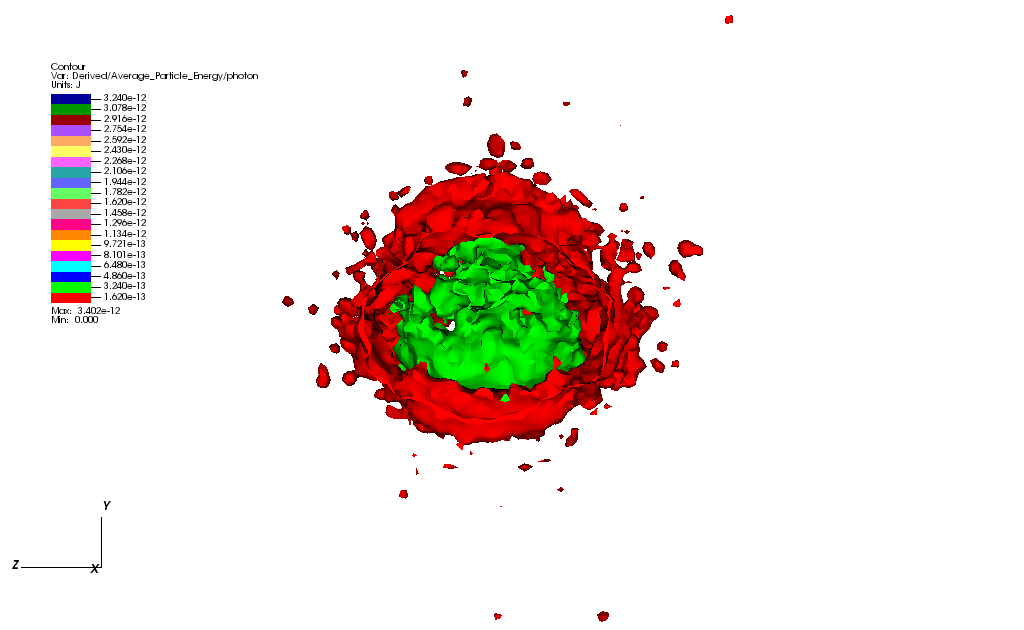
\includegraphics[width=1.0\textwidth]{/thesis-pics/structured-target/photons/1microns_in}
  \end{subfigure}
  \vskip\baselineskip
  \begin{subfigure}[b]{0.47\textwidth}
    \centering
    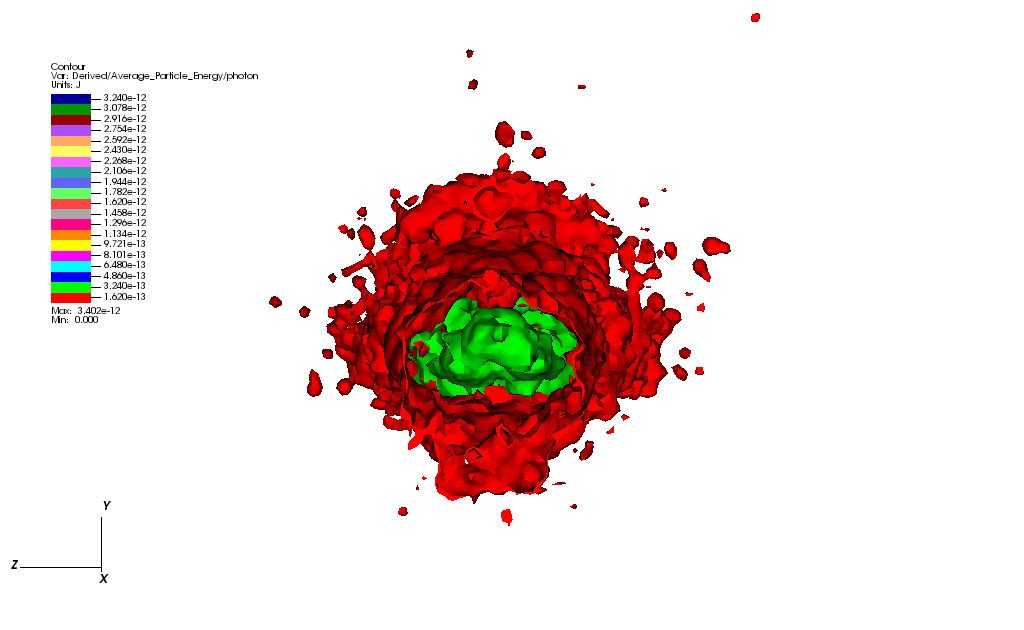
\includegraphics[width=1.0\textwidth]{/thesis-pics/structured-target/photons/3microns_in}
  \end{subfigure}
  \hfill
  \begin{subfigure}[b]{0.47\textwidth}
    \centering
    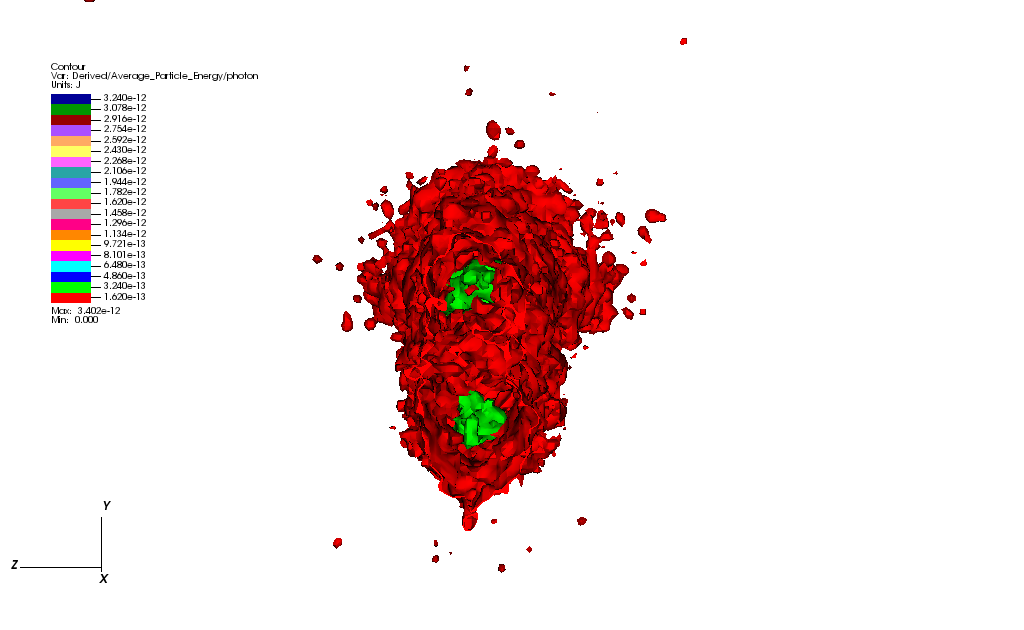
\includegraphics[width=1.0\textwidth]{/thesis-pics/structured-target/photons/6microns_in}
  \end{subfigure}
  \caption{A series of contour plots of the average photon energy showcasing all the photons produced up to 100fs into the simulation. Different plots show different clips of the photon bulk. They are displayed in the following order: top left - uncut view; top right - cut through the middle in the x-z plane; middle left - cut through the middle in the x-y plane; middle right - transversal cut 1 \(\mu\)m in from the entry plane of the laser; bottom left - - transversal cut 3 \(\mu\)m in from the entry plane of the laser; bottom right - transversal cut 6 \(\mu\)m in from the entry plane of the laser.}%
  \label{fig:photons}%
\end{figure}

\begin{figure}[!h]
  \centering
  \includegraphics[width=1.0\textwidth]{/thesis-pics/structured-target/1PW/visit0001}%
  \caption{A plot of the electron number density 100 fs into the simulation that showcases how the passage of the laser through the plasma affects the sructure of our plasma pipe. Some channel electrons spread inside the bulk region.}
  \label{fig:electron-current}%
\end{figure}

In order to compare the photon production as a function of channel radius, we look at the average particle energy per grid cell. We count all the cells that contain an average energy larger than a certain lower limit. The results are shown in~\cref{fig:efficiency}. In this plot, by efficiency we actually mean the number of grid cell with average energy above a ceratain value divided by the total number of grid cells that contain non-zero values of photon energy. This is used as a way to estimate the fraction of photons above certain energies from the total number of photons produced in the simulation. We can see that both graphs show an increase with the increase of the channel radius. This trend is more pronounced in the low energy samples. We also note that the cuves are concave, which suggests that further increase of the channel radius will not continue to increase the synchrotron photon yield. This is expected, since further increase in the radius would make the channel much thicker than the laser beam.

\begin{figure}[!h]
  \centering
  \begin{subfigure}[t]{0.9\textwidth}
    \centering
    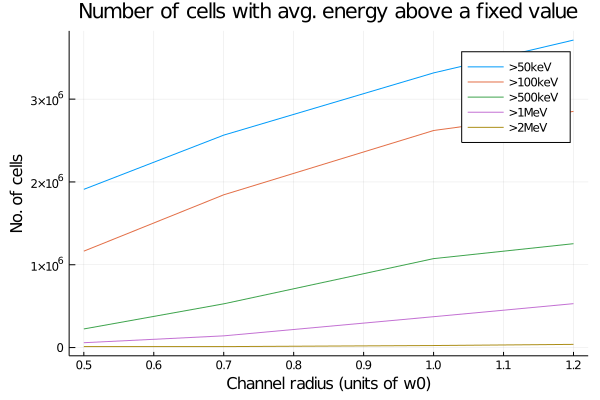
\includegraphics[width=1.0\textwidth]{/thesis-pics/structured-target/energies}
  \end{subfigure}
  \hfill
  \begin{subfigure}[t]{0.9\textwidth}
    \centering
    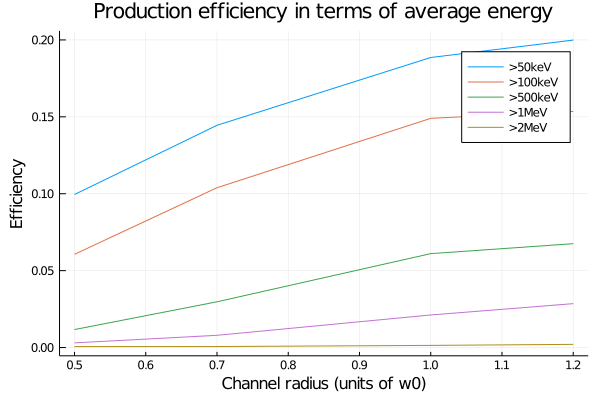
\includegraphics[width=1.0\textwidth]{/thesis-pics/structured-target/efficiency}
  \end{subfigure}
  \caption{Plots comparing the production yield of different photon energies in terms of the channel radius. Top: the number of cells with average photon energy above 50 keV, 100 keV, 500 keV, 1 Mev, and 2 MeV, respectively. Bottom: the production efficiency for different energies above the same lower limits as in the previous plot.}%
  \label{fig:efficiency}%
\end{figure}

\end{document}
